\begin{figure}
\centering
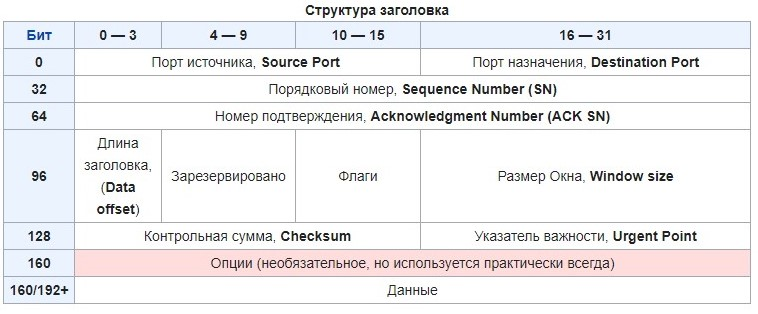
\includegraphics{./files/tcp_header_scheme.jpg}
\caption{Заголовок сегмента TCP}
\end{figure}

\textbf{Описание содержимого TCP заголовка:}

\begin{itemize}
\item
  \textbf{Порт источника} - номер порта из которого был отправлен пакет,
  ответ формируется по порту источника.
\item
  \textbf{Порт назначение} - номер порта на который был отправлен пакет.
\item
  \textbf{Порядковый номер} (\textbf{SYN}) - число полезные переданных
  данных в байтах. При установленном флаге SYN поле будет содержать
  начальный порядковый номер (ISN) - случайно сгенерированное число, а
  первый байт полезных данных в сессии будет иметь номер ISN+1.
\item
  \textbf{Номер подтверждения} (\textbf{ACK SN}) - при установленном
  флаге ACK, поле содержит номер октета, который отправитель хочет
  получить. Так же это значит что октеты от ISN+1 до ACK-1 были успешно
  получены.
\item
  \textbf{Длина заголовка} - смещение полезных данных относительно
  начала пакета.
\item
  Поле \textbf{зарезервировано} и \textbf{флаги} - 12 бит выделенные под
  различные флаги (ACK,SYN и др.), а так же зарезервированное
  пространство для будущих флагов.
\item
  \textbf{Размер окна} - количество байт полезны данных после передачи
  которых отправитель будет ожидать подтверждение получения.
\item
  \textbf{Контрольная сумма} - сумма всех 16 битных слов заголовка и
  данных. Если сегмент не кратен 16 битам то он дополняется нулями. Само
  поле в момент расчета суммы принимается равным нулю.
\item
  \textbf{Указатель важности} - используется для передачи внеполосных
  данных.
\end{itemize}

\hypertarget{ux43fux440ux43eux442ux43eux43aux43eux43b-udp}{%
\subsubsection{Протокол
UDP}\label{ux43fux440ux43eux442ux43eux43aux43eux43b-udp}}

\textbf{UDP} - протокол транспортного для работы с датаграммами,
расширяет IP добавлением в заголовок полей: порт отправителя, порт
получателя, длина датаграммы и контрольной суммы.
